
\documentclass[9pt]{beamer}
%\makeatletter
%\def\beamer@calltheme#1#2#3{%
%	\def\beamer@themelist{#2}
%	\@for\beamer@themename:=\beamer@themelist\do
%	{\usepackage[{#1}]{\beamer@themelocation/#3\beamer@themename}}}
%
%\def\usefolder#1{
%	\def\beamer@themelocation{#1}
%}
%\def\beamer@themelocation{}

%\usefolder{../config}

\usetheme[
block=fill,
titleformat=regular,
progressbar=frametitle
]{metropolis}
%\metroset[everytitleformat=regular] % regular, lowercase, uppercase ]
%\metroset[inner/block=fill]

%\setbeameroption{show notes} 
\usepackage{booktabs}
\usepackage[scale=2]{ccicons}

\usepackage{pgfplots}
\usepgfplotslibrary{dateplot}


%\ Hrvatski znakovi
\usepackage[utf8]{inputenc}
\usepackage[T1]{fontenc}
\usepackage[croatian]{babel}
\usepackage{todonotes}
\usepackage{amsmath}
\usepackage{amsfonts}
\selectlanguage{croatian} % american ngerman
\usepackage{todonotes}

% Koristenje Latin modern fonta
% Bez toga na nekim racunalima baca
% err: Font <taj i taj> at <mala velicina, npr4.0pt> not loadable: Metric (TFM) file not found. \end{frame}
\usepackage{lmodern}


\definecolor{RoyalBlue}{cmyk}{1, 0.50, 0, 0}
%\usepackage{natbib}
%\usepackage{bibentry}
\usepackage{scrextend}
\usepackage{hyperref}
%\usepackage[pdfa=true]{hyperref}
\hypersetup{%
    %draft, % = no hyperlinking at all (useful in b/w printouts)
    %colorlinks=true, 
    linktocpage=true, pdfstartpage=3, pdfstartview=FitV,%
    % uncomment the following line if you want to have black links (e.g., for printing)
    %colorlinks=false, linktocpage=false, pdfborder={0 0 0}, pdfstartpage=3, pdfstartview=FitV,% 
    breaklinks=true, pdfpagemode=UseNone, pageanchor=true, pdfpagemode=UseOutlines,%
    plainpages=false, bookmarksnumbered, bookmarksopen=true, bookmarksopenlevel=1,%
    hypertexnames=true, pdfhighlight=/O,%nesting=true,%frenchlinks,%
    %urlcolor=webbrown, linkcolor=RoyalBlue, citecolor=webgreen, %pagecolor=RoyalBlue,%
    %urlcolor=Blue, linkcolor=Blue, citecolor=Red, %pagecolor=Black,%
    %pdftitle={\myTitle},%
    %pdfauthor={\textcopyright\ \myName, \myUni, \myFaculty},%
    pdfsubject={},%
    pdfkeywords={},%
    pdfcreator={pdfLaTeX},%
    pdfproducer={LaTeX with hyperref and classicthesis}, %
    unicode = true 
} 

%\usepackage[pdftex]{graphicx}
% declare the path(s) where your graphic files are
\graphicspath{{./}{./figures/}}


\newcommand{\executeiffilenewer}[3]{%
	\ifnum\pdfstrcmp{\pdffilemoddate{#1}}%
	{\pdffilemoddate{#2}}>0%
	{\immediate\write18{#3}}\fi%
}
\newcommand{\includesvg}[1]{%
	\executeiffilenewer{#1.svg}{#1.pdf}%
	{inkscape -z -C --file=#1.svg %
		--export-pdf=#1.pdf --export-latex}%
	\input{#1.pdf_tex}%
}


% http://tex.stackexchange.com/questions/83882/how-to-highlight-python-syntax-in-latex-listings-lstinputlistings-command

\usepackage{listings}
\usepackage{color}
\usepackage[semibold]{sourcecodepro}

% Default fixed font does not support bold face
\DeclareFixedFont{\ttb}{T1}{txtt}{bx}{n}{12} % for bold
\DeclareFixedFont{\ttm}{T1}{txtt}{m}{n}{12}  % for normal
% Custom colors
\definecolor{deepblue}{rgb}{0,0,0.5}
\definecolor{deepred}{rgb}{0.6,0,0}
\definecolor{deepgreen}{rgb}{0,0.5,0}


% Python style for highlighting
\newcommand\pythonstyle{\lstset{
		language=Python,
		basicstyle=\small\ttfamily,
		otherkeywords={self},             % Add keywords here
		keywordstyle=\small\ttfamily\color{deepblue},
		emph={MyClass,__init__},          % Custom highlighting
		emphstyle=\small\ttfamily\color{deepred},    % Custom highlighting style
		stringstyle=\color{deepgreen},
		frame=tb,                         % Any extra options here
		showstringspaces=false            % 
	}}
	
	
	% Python environment
	\lstnewenvironment{python}[1][]
	{
		\pythonstyle
		\lstset{#1}
	}
	{}
	
	% Python for external files
	\newcommand\pythonexternal[2][]{{
			\pythonstyle
			\lstinputlisting[#1]{#2}}}
	
	% Python for inline
	\newcommand\pythoninline[1]{{\pythonstyle\lstinline!#1!}}
%\documentclass[ucs]{beamer}
%\usetheme[menuwidth={0.3\paperwidth}]{erlangen}
%\setbeamercovered{transparent=20} 

\usepackage{amsmath,amsfonts,amsthm,amssymb}
\usepackage{setspace}
\usepackage{Tabbing}
\usepackage{fancyhdr}
\usepackage{lastpage}
\usepackage{extramarks}
\usepackage{chngpage}
\usepackage{soul,color}
\usepackage{graphicx,float,wrapfig}
\usepackage{xcolor}
\usepackage[normalem]{ulem}
\usepackage{mathtools}
\usepackage{cancel}

\definecolor{erlangenlyellow}{RGB}{123, 25, 121}
%\usepackage[utf8x]{inputenc}
%\usepackage{default}
%\usepackage[T1]{fontenc}

\usepackage{verbatim}
\usepackage{listings}
\usepackage{algorithm2e}


\usepackage{subcaption}
\usepackage{lmodern}

\title{Ray tracing}

\subtitle{Ray tracing is the future and ever will be\ldots - David Kirk}
\institute{Računalna grafika}

% Delete this, if you do not want the table of contents to pop up at
% the beginning of each subsection:
%\AtBeginSubsection[]
%{
%  \begin{frame}<beamer>{Outline}
%    \tableofcontents[currentsection,currentsubsection]
%  \end{frame}
%}
%
%\AtBeginSection[]
%{
%  \begin{frame}<beamer>{Outline}
%    \tableofcontents[currentsection]
%  \end{frame}
%}

\begin{document}
\begin{frame}
 \titlepage
\end{frame}

\begin{frame}{Sadržaj}
  \tableofcontents
  % You might wish to add the option [pausesections]
\end{frame}


\section{Algoritam bacanja zrake - ray casting}
\begin{frame}{Uvod}
\begin{itemize}
	\item Poznat još od početka 70-ih
	\item Izrazito jednostavan
	\item Danas osnovni alat
\end{itemize}
\end{frame}

\begin{frame}{Ray casting}
\begin{itemize}
	\item Za svaki piksel
	\begin{itemize}
		\item Kreirati zraku od promatrača
		\item Za svaki objekt u sceni
		\begin{itemize}
			\item Naći sjecište sa zrakom
			\item Zadržati najbliže
			\item Sjenčanje - ovisi o svjetlu i normali
		\end{itemize}
	\end{itemize}
\end{itemize}
\begin{figure}
	 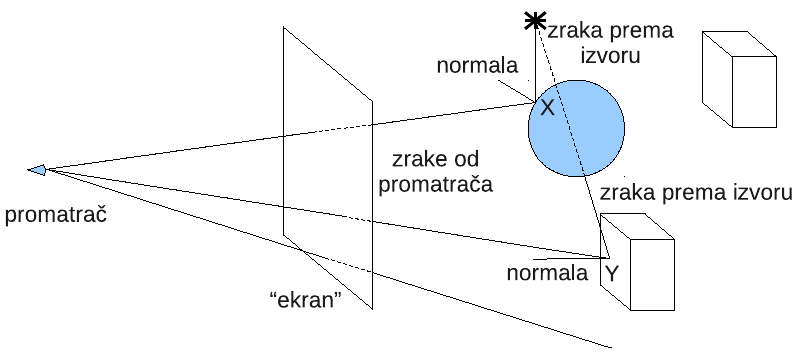
\includegraphics[width=0.6\textwidth]{./slike/model_bacanja_zrake.png}
	 \caption{Model bacanja zrake}
\end{figure}
\end{frame}	

\begin{frame}{Ray casting osnove}
\begin{block}{Generiranje primarne zrake}
	\begin{itemize}
		\item Zrake iz očišta kroz uzorkovane točke na ravnini
		\item Uzorkovana točka je centar piksela
	\end{itemize}
\end{block}
\begin{block}{Sjecište zrake i objekta}
	\begin{itemize}
		\item Naći prvi objekt u sceni s kojim se siječe zraka (ako sjecište postoji)
	\end{itemize}
\end{block}
\end{frame}

\begin{frame}{Ray casting algoritam}
\begin{algorithm*}[H]
	%\KwResult{Write here the result }
	\For{ za svaki slikovni element (x,y)}
	{
		izračunaj zraku od oka do slikovnog elementa (x,y)\;
		izračunaj sjecišta zrake sa svim objektima u sceni\;
		pronađi sjecište (i objekt) koje je najbliže\;
		\uIf{pronađi sjecište (i objekt) koje je najbliže}
		{
			dodijeli boju sjecištu (klasični model osvjetljavanja)\;
			zapiši tu boju slikovnom elementu (x,y)\;
		}\Else
		{
			postavi pozadinsku boju\;
		}
	}
\end{algorithm*}
\end{frame}

\begin{frame}{Ray casting algoritam}
\begin{itemize}
	\item Za svaki piksel
	\begin{itemize}
		\item \alert{Kreirati zraku od oka}
		\item Za svaki objekt u sceni
		\begin{itemize}
			\item Naći sjecište sa zrakom
			\item Zadržati najbližu
			\item Sjenčanje - ovisi o svjetlu i normali
		\end{itemize}
	\end{itemize}
\end{itemize}
\end{frame}

\begin{frame}{Ray casting algoritam}
\begin{figure}
	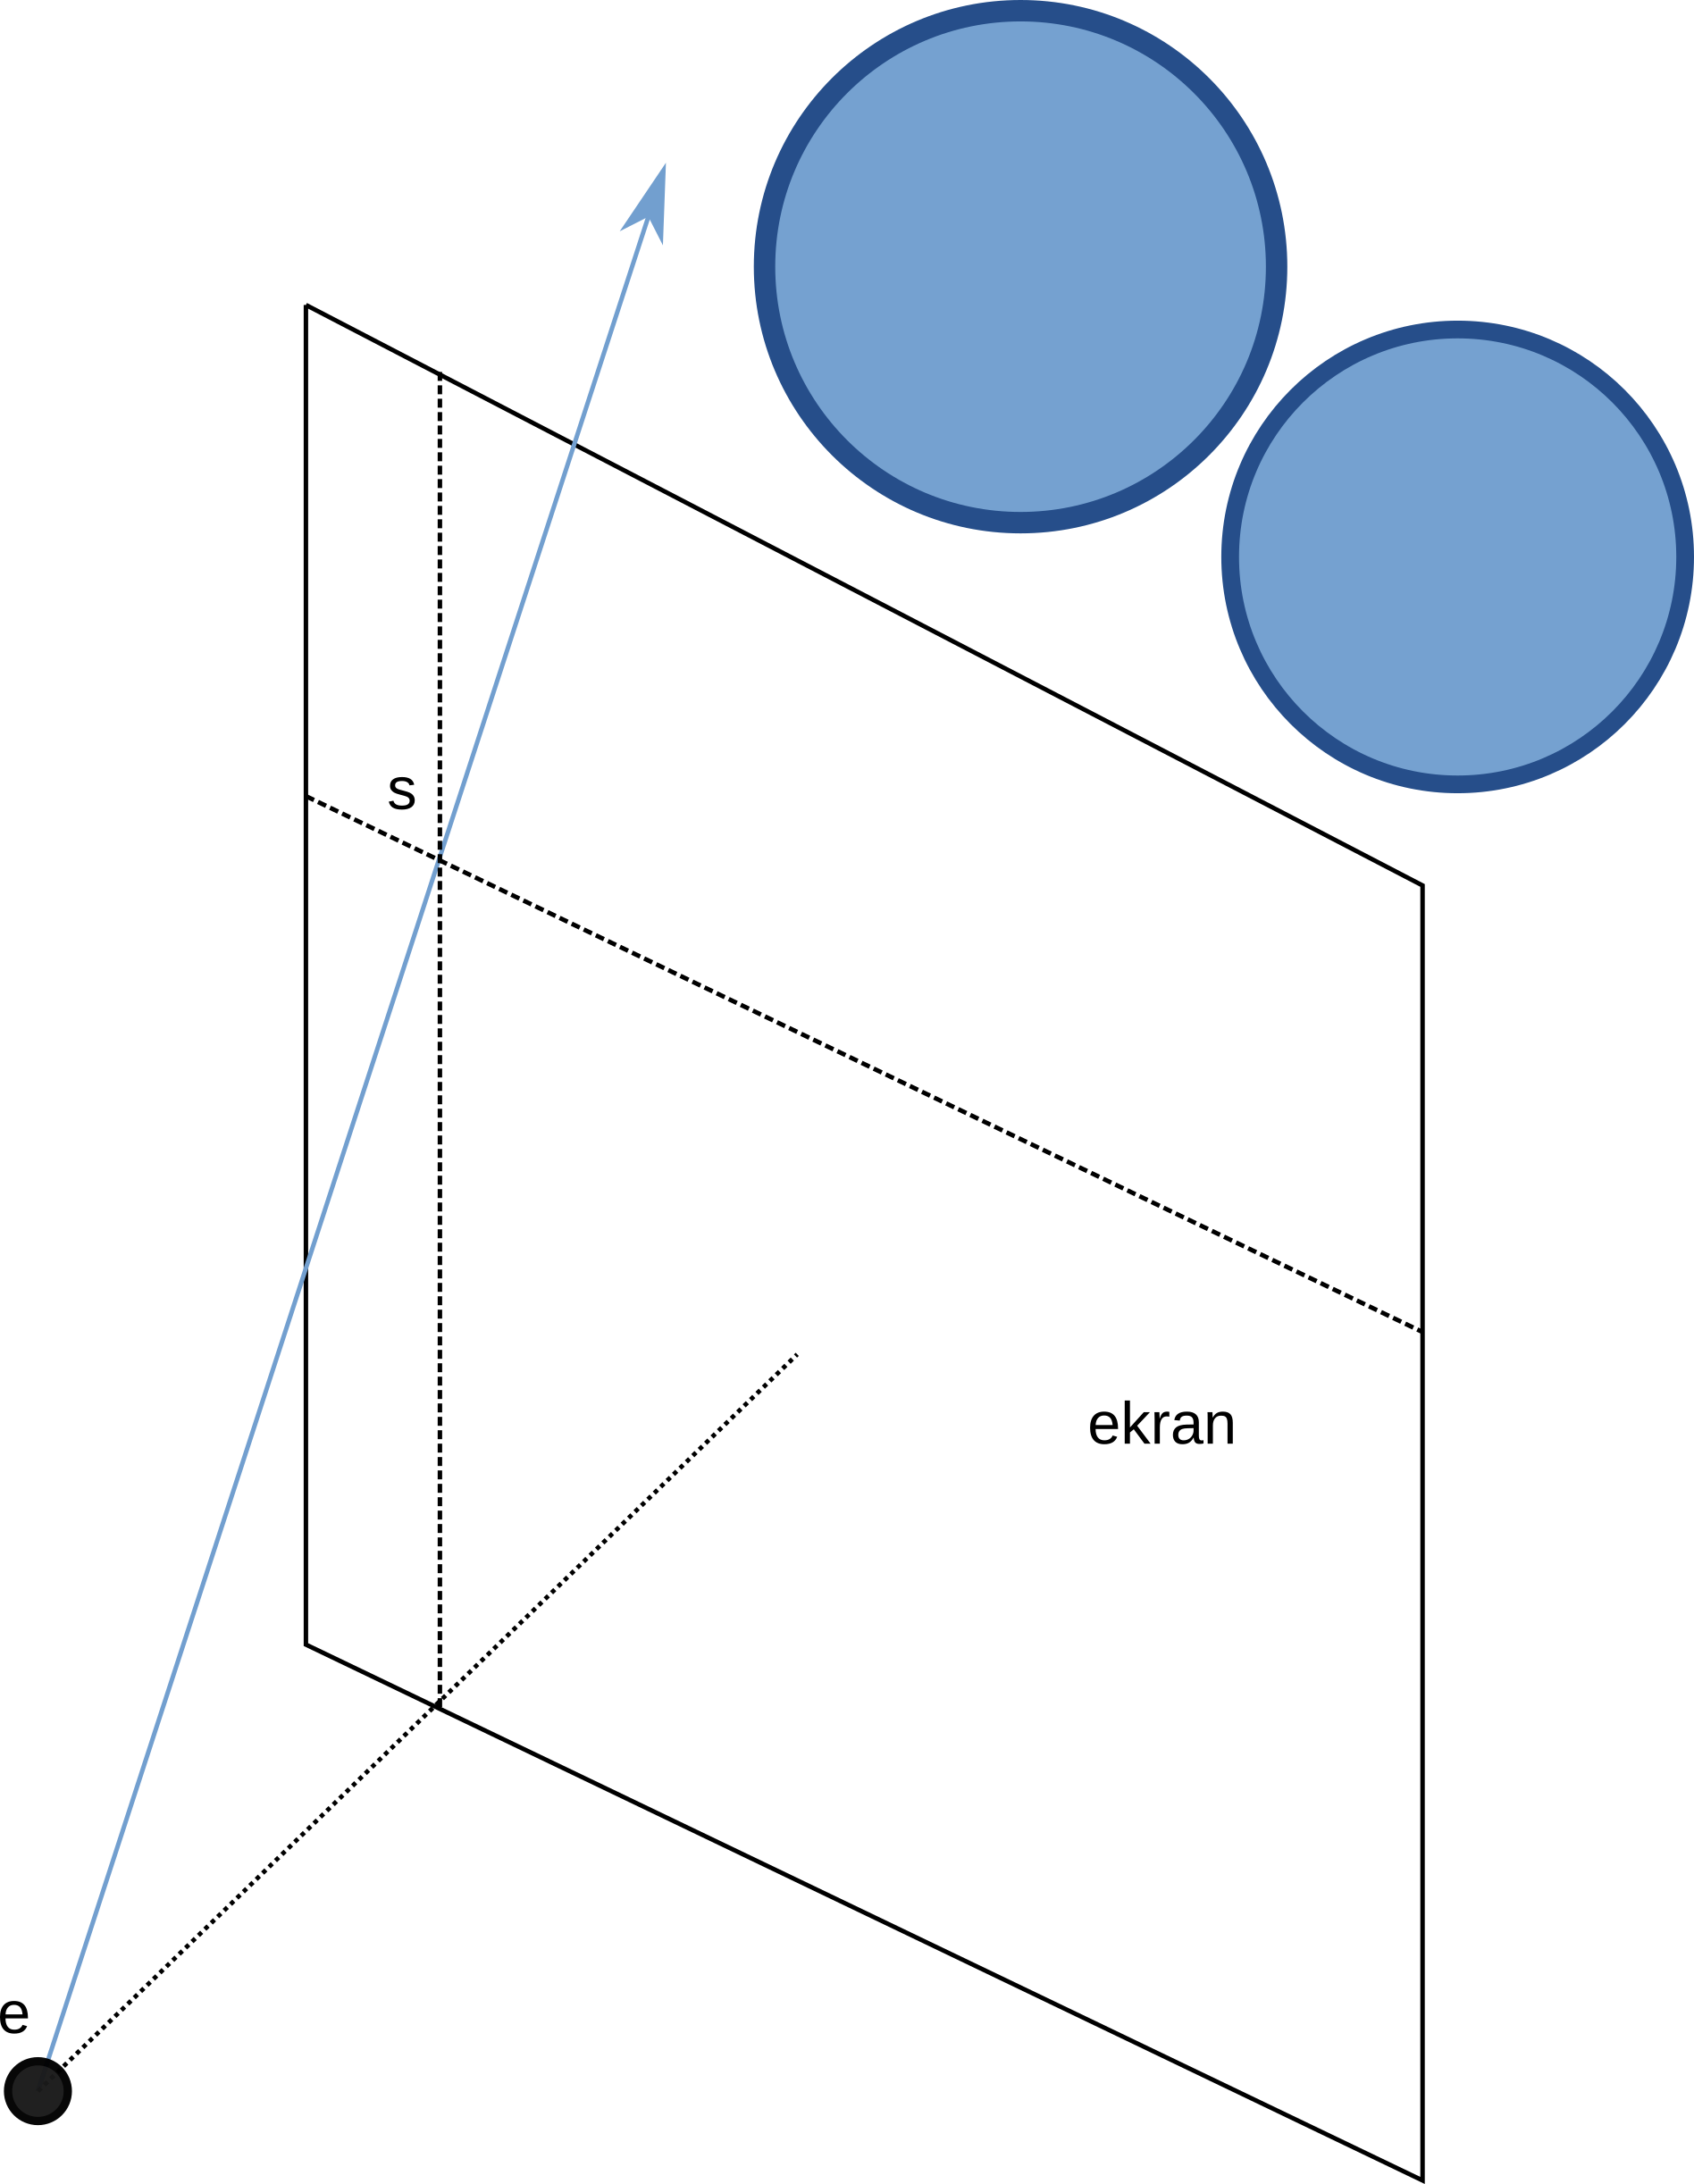
\includegraphics[width=0.4\textwidth]{./slike/zraka.png}
\end{figure}
\begin{align*}
	\textbf{p}(t) = \textbf{e} + t(\textbf{s} - \textbf{e})
\end{align*}
\end{frame}

\begin{frame}{Ray casting algoritam}
\begin{itemize}
	\item Za svaki piksel
	\begin{itemize}
		\item Kreirati zraku od oka
		\item \alert{Za svaki objekt u sceni}
		\begin{itemize}
			\item Naći sjecište sa zrakom
			\item Zadržati najbližu
			\item Sjenčanje - ovisi o svjetlu i normali
		\end{itemize}
	\end{itemize}
\end{itemize}
\end{frame}

\begin{frame}{Ray casting algoritam}
\begin{figure}
	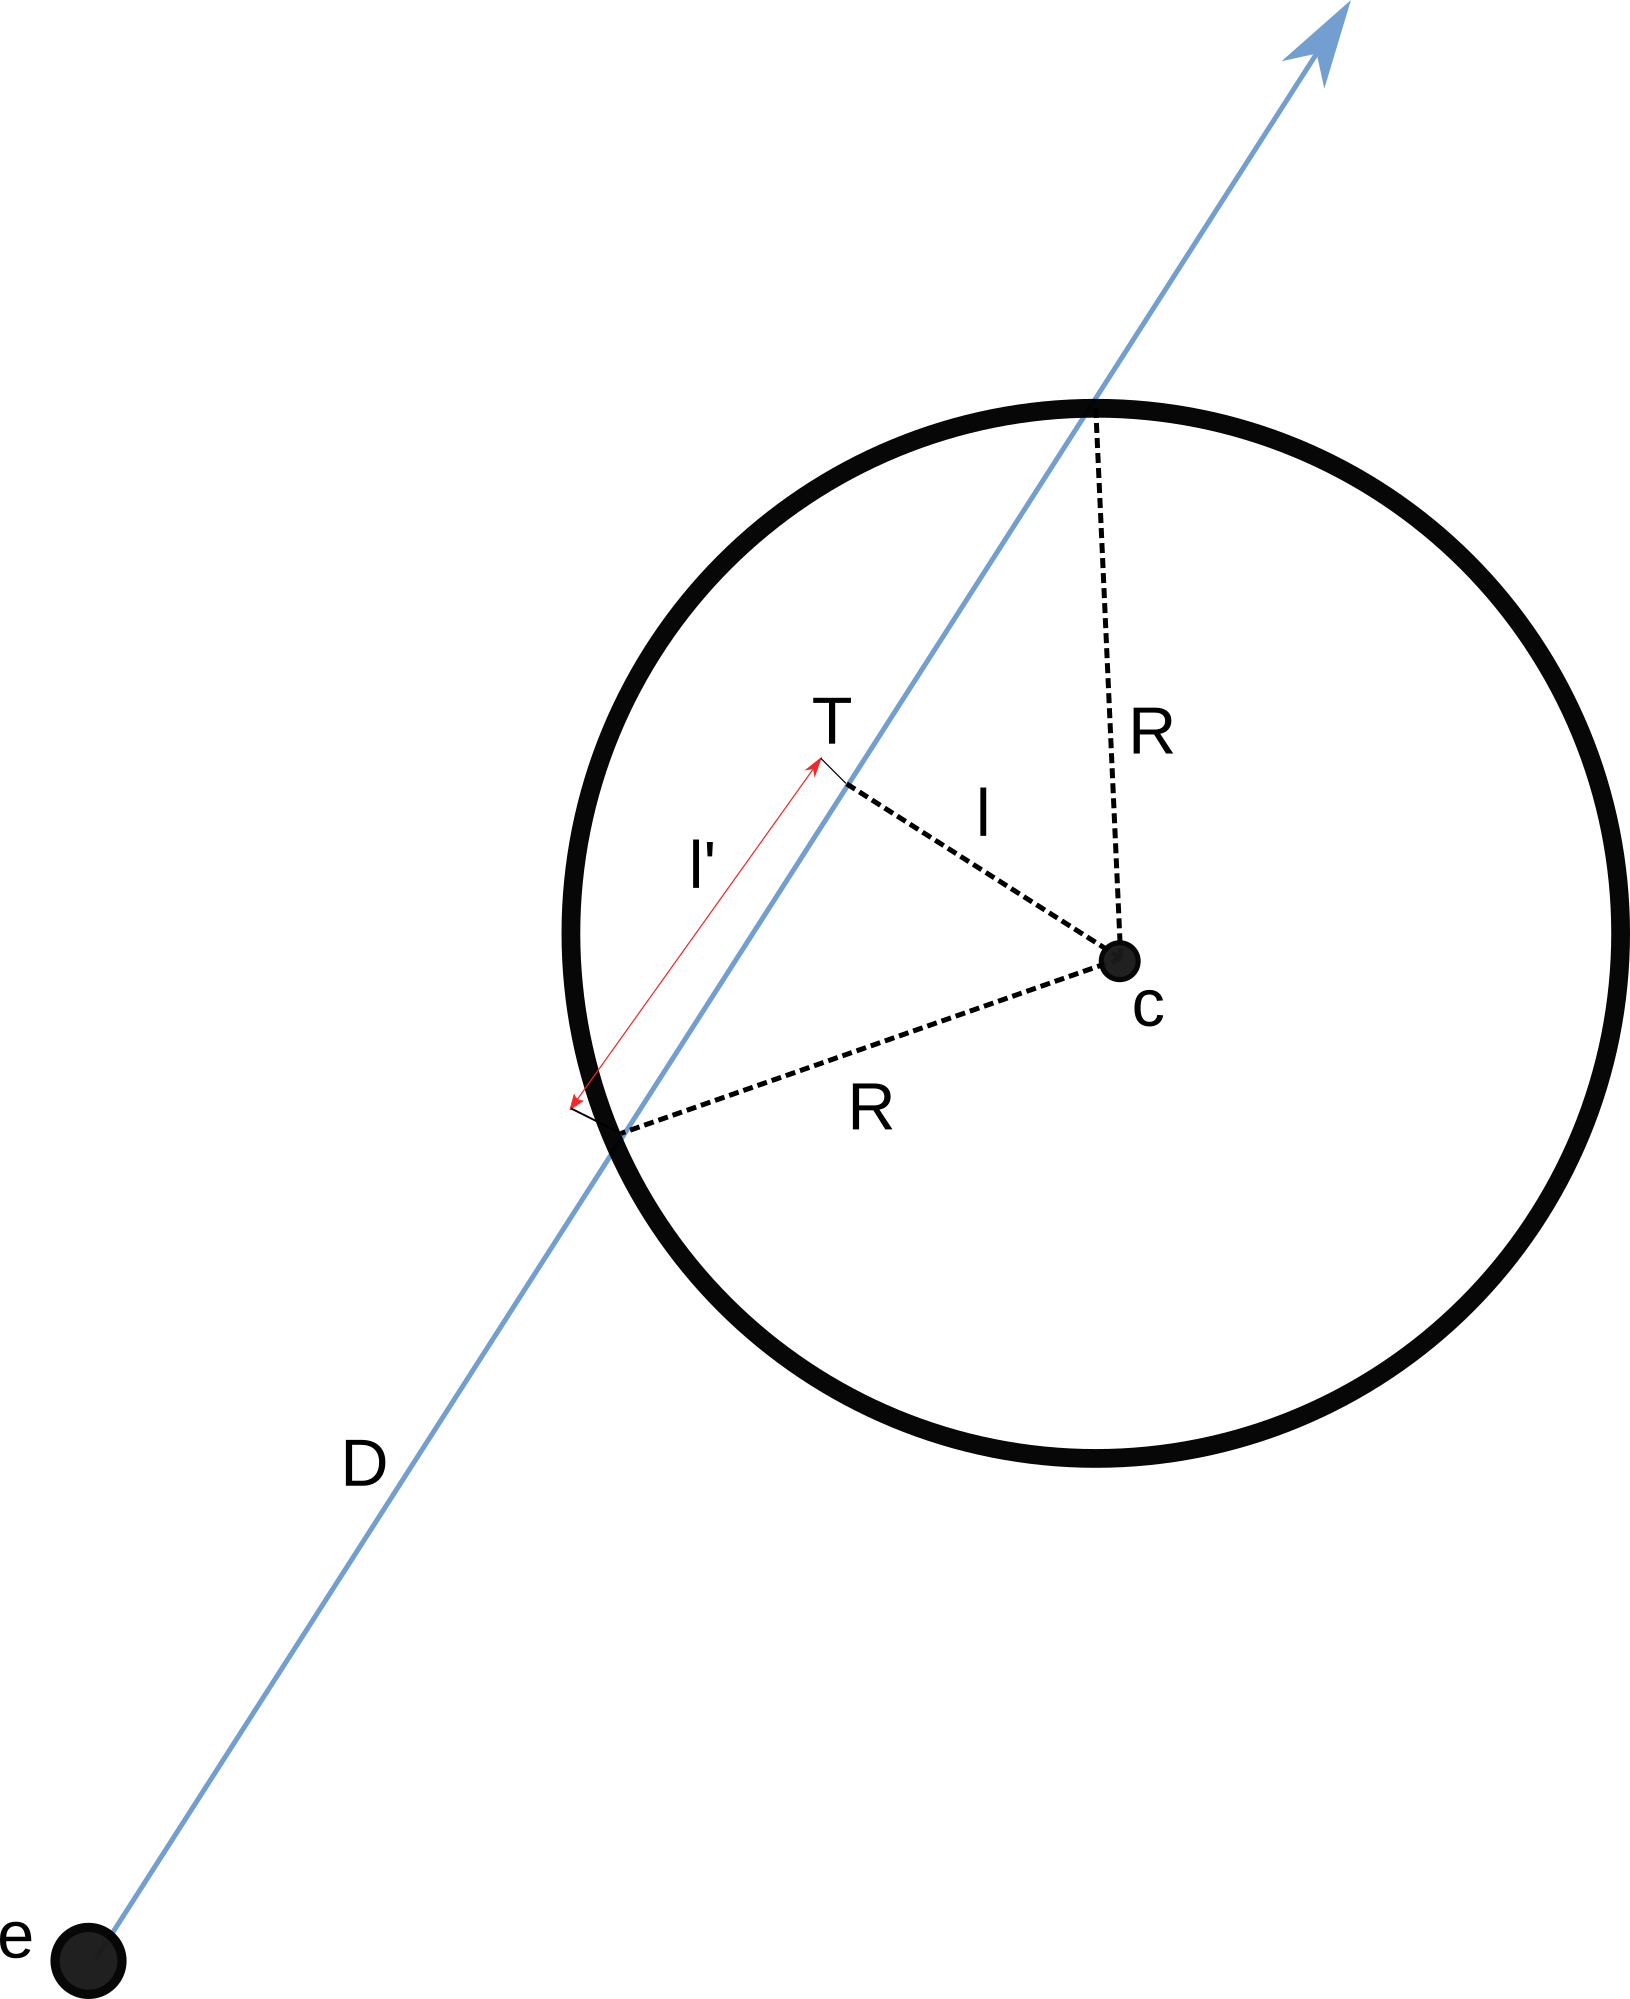
\includegraphics[width=0.4\textwidth]{./slike/sjeciste_kugla.png}
\end{figure}
\begin{itemize}
	\item $\vec{l}$ je okomit vektor na $\textbf{D}$
	\item Ako je $||\vec{l}|| > R$, nema sjecišta
	\item Ako je $||\vec{l}|| < R$, samo treba izračunati $l'$
	\item Zadržati bližu točku
\end{itemize}
\end{frame}

\begin{frame}{Ray casting algoritam}
\begin{columns}
	\begin{column}{0.5\textwidth}
		\begin{figure}
			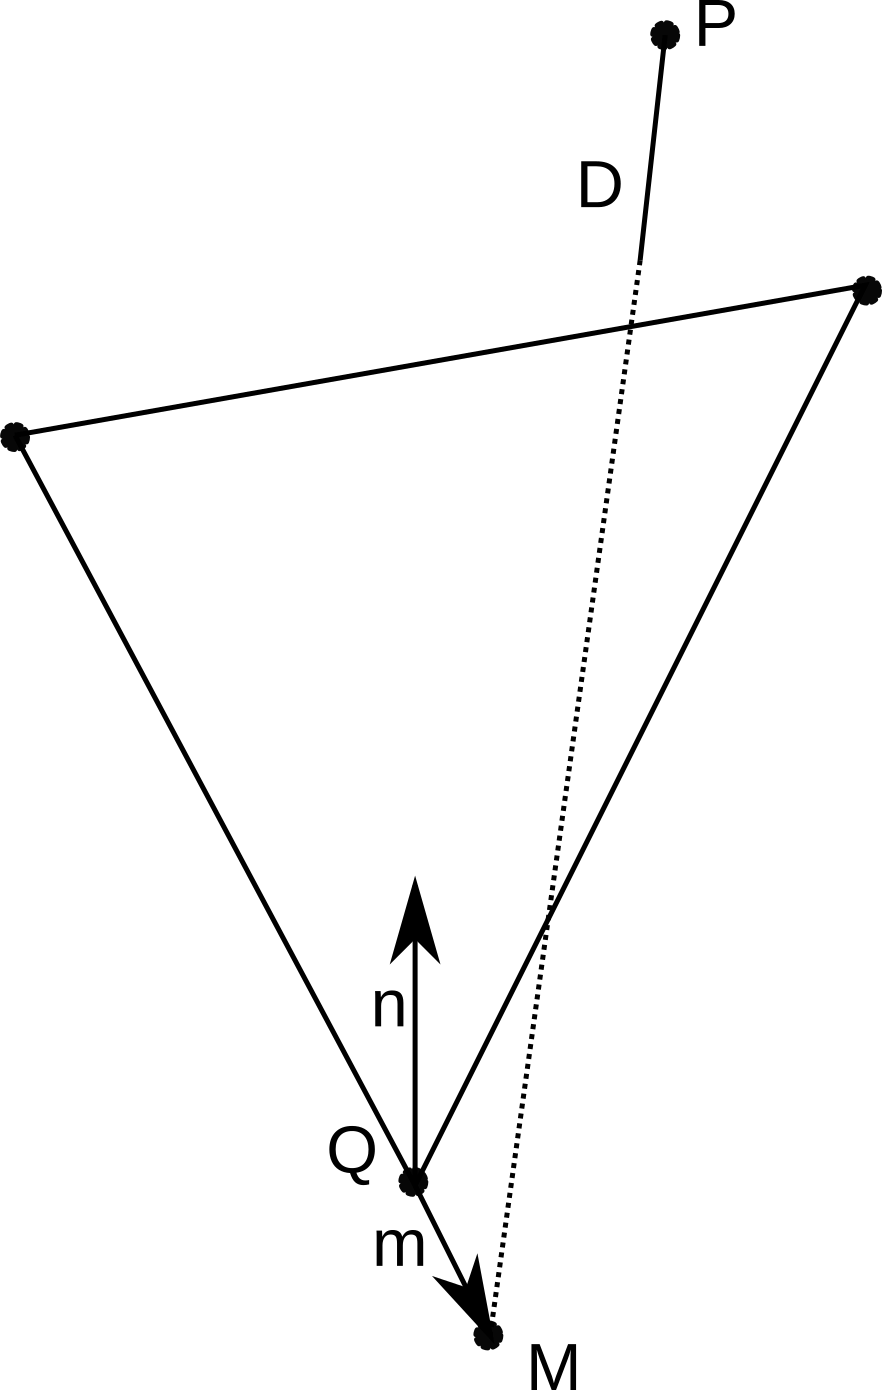
\includegraphics[width=0.5\textwidth]{./slike/trokut.png}
		\end{figure}
	\end{column}
	\begin{column}{0.5\textwidth}  %%<--- here
		\begin{itemize}
			\item $\vec{m}$ i $\vec{n}$ su okomiti vektori: $\vec{m}\cdot\vec{n}=0$
			\item $M = P+t\textbf{D}$
			\item $\vec{m} = M-Q$
			\item $\left(P+t\textbf{D}\right)\cdot \vec{n}=0$
			\item $t\textbf{D}\cdot\vec{n} + \left(P-Q\right)\cdot \vec{n}=0$
		\end{itemize}
		\begin{align*}
		t = \frac{-\left(P-Q\right)\cdot\vec{n}}{\textbf{D}\cdot \vec{n}}
		\end{align*}
		\begin{itemize}
			\item $\textbf{D}\cdot \vec{n}=0$, 
			\item $\textbf{D} \perp \vec{n}$
			\item nema sjecišta, jer je ravnina paralelna sa zrakom
		\end{itemize}
	\end{column}
\end{columns}
\end{frame}

\begin{frame}{Ray casting algoritam}

\begin{figure}
	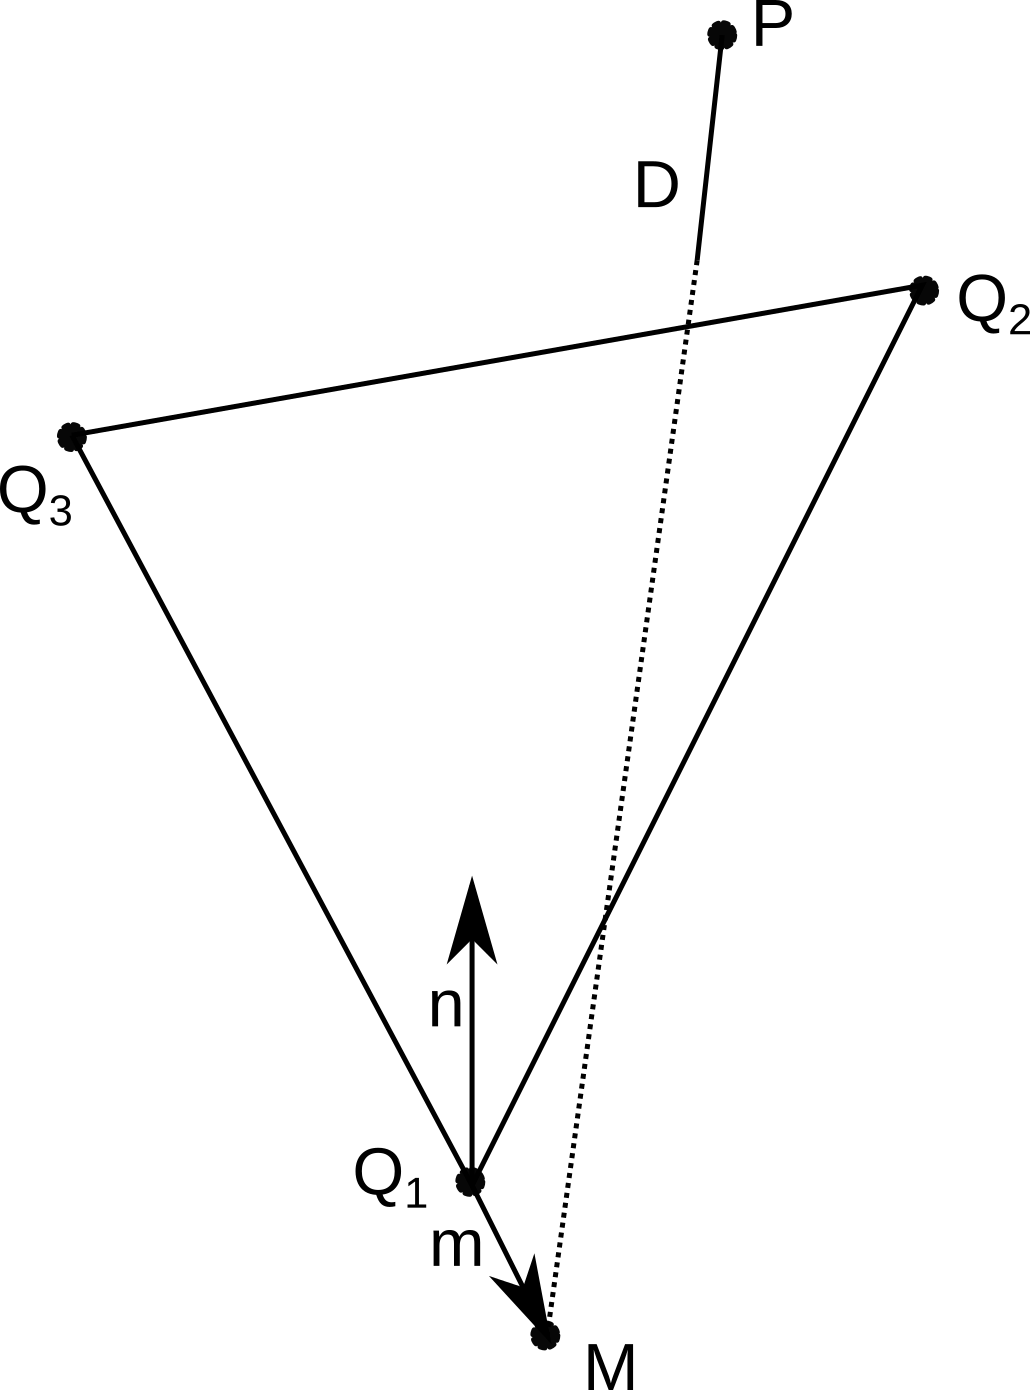
\includegraphics[width=0.4\textwidth]{./slike/trokut2.png}
\end{figure}
\begin{itemize}
	\item Nakon što dobijemo $M$
\end{itemize}
\begin{align*}
M = \alpha Q_1 + \beta Q_2 + \gamma Q_3 \\
 \alpha + \beta + \gamma = 1
\end{align*}
\end{frame}

\begin{frame}{Ray casting algoritam}
\begin{itemize}
	\item Za svaki piksel
	\begin{itemize}
		\item Kreirati zraku od oka
		\item Za svaki objekt u sceni
		\begin{itemize}
			\item Naći sjecište sa zrakom
			\item Zadržati najbližu
			\item \alert{Sjenčanje - ovisi o svjetlu i normali}
		\end{itemize}
	\end{itemize}
\end{itemize}
\end{frame}

\begin{frame}{Ray casting algoritam}
\begin{figure}
	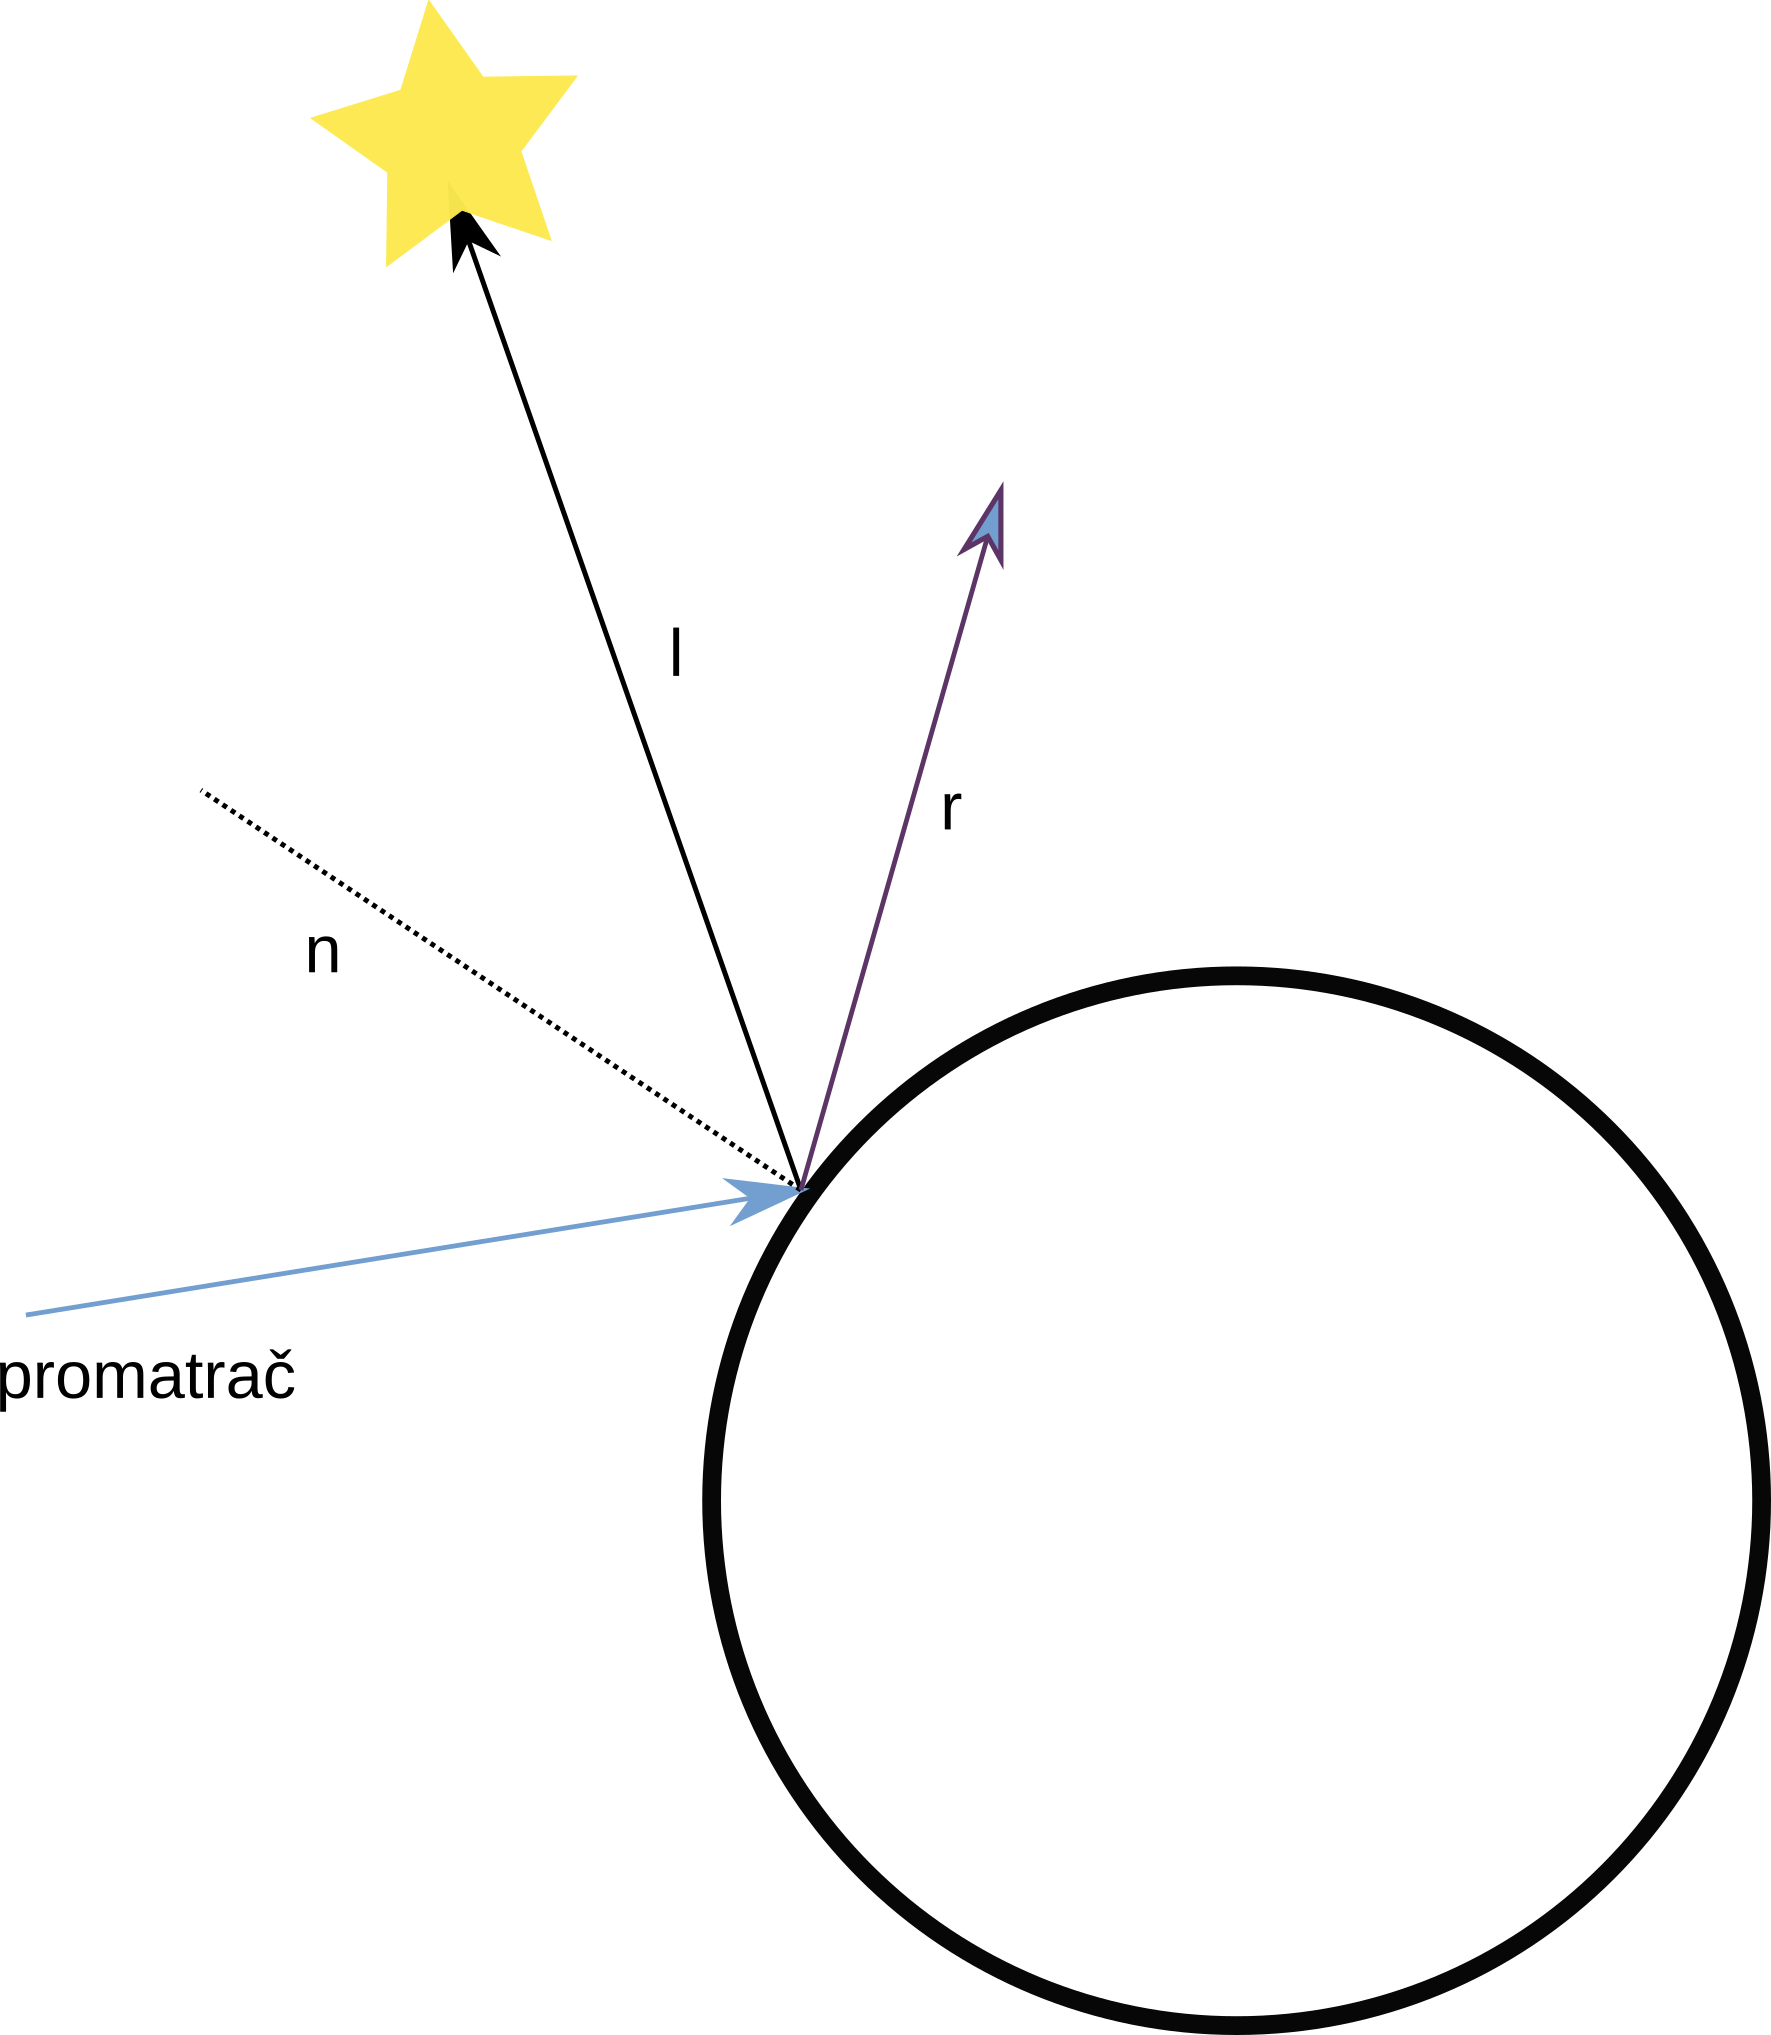
\includegraphics[width=0.4\textwidth]{./slike/sjencanje.png}
\end{figure}
\begin{align*}
I = k_aI_a + I_i\left[k_d\left(\mathbf{n}\cdot\mathbf{l}\right)+
k_s\left(\mathbf{v}\cdot\mathbf{r}\right)^q\right]
\end{align*}
\end{frame}
\section{Kreiranje primarne zrake}
\begin{frame}{Kreiranje primarne zrake}
\begin{center}
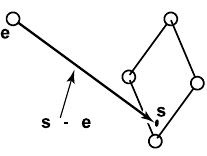
\includegraphics[width=3cm]{slike/ray_from_eye.png}
\end{center}
Ovdje je $\textbf{e}$ položaj očišta, a $\textbf{s}$ koordinata na "image plane".
Jednadžba zrake: 
$$\textbf{p}(t) = \textbf{e} + t(\textbf{s} - \textbf{e})$$
\begin{itemize}
\item $t<0$ - $\textbf{p}(t)$ leži na pravcu iza očišta
\item $t=0$, ili $\textbf{p}(0) = \textbf{e}$
\item $t=1$, ili $\textbf{p}(1) = \textbf{s}$
\end{itemize}
\end{frame}

\begin{frame}{Kreiranje primarne zrake, contd.}
Kako postaviti kameru?
\begin{center}
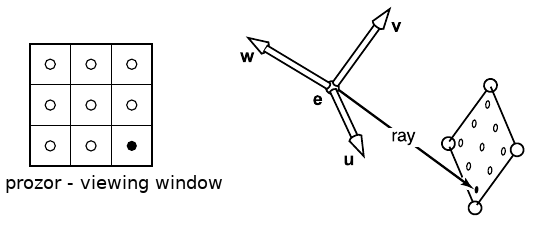
\includegraphics[width=5cm]{slike/ray_viewing_window.png}\quad 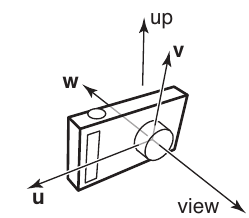
\includegraphics[width=2cm]{slike/ray_camera.png}
\end{center}

Ako znamo $\textbf{e}$, ako definiramo \textit{up vector}($\textbf{up}$) i odredimo smjer gledanja $\textbf{D}$, gdje je $d=||\textbf{D}||$ udaljenost prozora od očišta:
\begin{itemize}
\item $\textbf{w} = -\textbf{D}$
\item $\textbf{u} = \textbf{w}\times \vec{up}$
\item $\textbf{v} = \textbf{w}\times \textbf{u}$
\end{itemize}
Svi vektori $\textbf{u}$, $\textbf{v}$ i $\textbf{w}$ moraju biti normalizirani (duljine 1).
\begin{align*}
\textbf{w} = \frac{\textbf{w}}{||\textbf{w}||} \quad \textbf{u} = \frac{\textbf{u}}{||\textbf{u}||} 
\quad \textbf{v} = \frac{\textbf{v}}{||\textbf{v}||}
\end{align*}

\end{frame}

\begin{frame}{Kreiranje primarne zrake, contd.}
Kako  odrediti poziciju na prozoru?
\begin{figure}
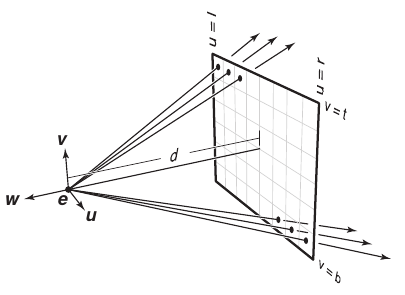
\includegraphics[width=0.4\textwidth]{slike/ray_viewing_window_perspective.png} 
\end{figure}
Udaljenost od promatrača $d$ definiramo $d = -w$
Ako prozor sadrži $(n_x,n_y)$ piksela, potrebno je izraziti poziciju $(i,j)$ u $(u,v)$ koordinatnom sustavu (ovdje $t$ označava \textit{top}, gornju koordinatu prozora):
$$n_x \cdot n_y = (r-l) \cdot (t-b)$$
$$
u = \frac{l + (r-l)(i+1/2)}{n_x}\quad v = \frac{b + (t-b)(j+1/2)}{n_y}
$$
Ovdje je $1/2=0.5$, odnosno centar piksela
\end{frame}


\begin{frame}{Kreiranje primarne zrake, contd.}
Primjer:
\begin{align*}
l = -500, \quad r = 500, \quad n_x = 100, \quad i=25
\end{align*}
$$
u = \frac{l + (r-l)(i+1/2)}{n_x} = \frac{-500 + (500- (-500))(25+0.5)}{100}
$$
\end{frame}

\begin{frame}{Još jedan način kreiranja primarne zrake}
\begin{itemize}
	\item definiramo omjer stranica \textit{aspect ratio}, ili $ar = 16/9$
	\item visina prozora: $w_h = 2$
	\item širina prozora: $w_w = ar\cdot w_h$
	\item piksela po širini: $n_x = 384$
	\item piksela po visini: $n_y = n_x/ar$
\end{itemize}
\begin{columns}
	\begin{column}{0.5\linewidth}
		\begin{itemize}
			\item $d = 1$
			\item $\textbf{e}= (0, 0, 0)$
			\item $\textbf{w}_w= (w_w, 0, 0)$
			\item $\textbf{w}_h= (0, w_h, 0)$
		\end{itemize}
	\end{column}
	\begin{column}{0.5\linewidth}
		\begin{itemize}
			\item definiramo $i$, $j$, od $0$ do $n_x$, odnosno $n_y$
			\item $u= i/(n_x-1)$ \quad  $v= j/(n_y-1)$
			\item $\textbf{s} = (u, v, d)$
		\end{itemize}
	\end{column}
\end{columns}

\begin{figure}
	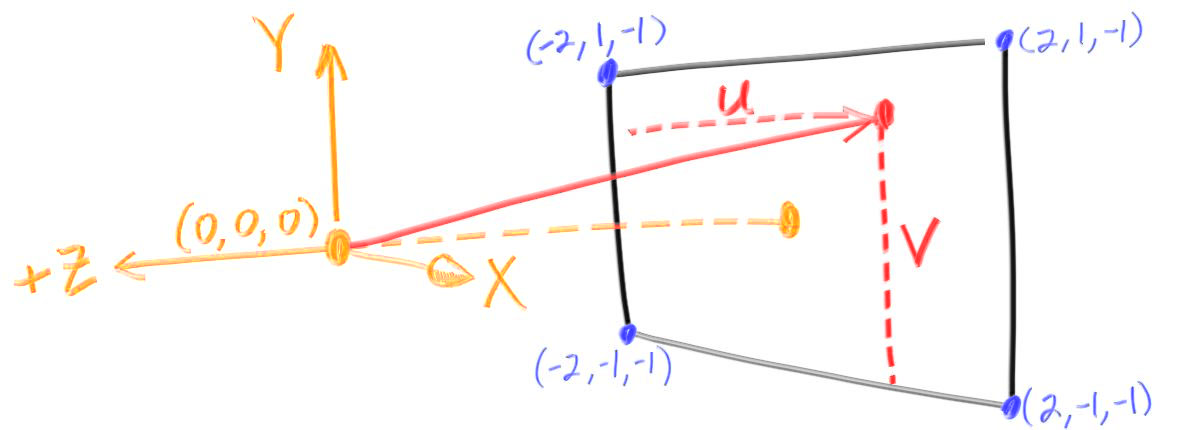
\includegraphics[width=0.5\linewidth]{./slike/fig-cam-geom.png}
\end{figure}
\end{frame}
\begin{frame}{Kreiranje primarne zrake, contd.}
\begin{center}
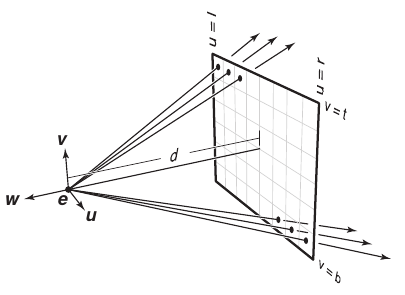
\includegraphics[width=4cm]{slike/ray_viewing_window_perspective.png} 
\end{center} 
Sada smo izračunali koordinate $(u,v, w)$. Potrebno je kreirati jednadžbu pravca:Imamo $\textbf{e}$, $d$, $(u,v, w)$.
$$\textbf{p}(t) = \textbf{e} + t(\textbf{s} - \textbf{e})$$
Kako je:
$$\textbf{s} - \textbf{e} = u\textbf{u} + v\textbf{v} - d\textbf{w}$$
onda slijedi:
$$\textbf{p}(t) = \textbf{e} + t(u\textbf{u} + v\textbf{v} - d\textbf{w})$$
\end{frame}

\begin{frame}{Kreiranje primarne zrake, contd.}
Ortografska projekcija:
\begin{center}
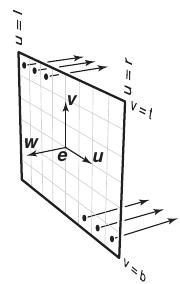
\includegraphics[width=1.8cm]{slike/ray_viewing_window_orthografic.png} 
\end{center} 
Smještamo centar \textit{viewing window}-a u očište ($\textbf{s} = \textbf{e}$), izračunamo $\textbf{u}$, $\textbf{v}$ i $\textbf{w}$, jer smo već zadali smjer gledanja $\textbf{D}$ i \textit{up vector} $\textbf{up}$.\\
Koordinate $(u,w)$ izračunamo kao i prije. Sada mijenjamo položaj očišta, a smjer gledanja nam je $\textbf{D}$.
$$\textbf{p}(t) = \textbf{e} + u\textbf{u} + v\textbf{v} - t\textbf{w}$$
Ovdje je ishodište u: $\textbf{e} + u\textbf{u} + v\textbf{v}$, a smjer:
$- t\textbf{w}$
\end{frame}
\section{Određivanje sjecišta}
\begin{frame}{Sjecište zrake i sfere}
Sfera:
$$(x-x_c)^2 + (y-y_c)^2 + (z-z_c)^2 - R = 0$$
Pravac:
$$\textbf{p}(t) = \textbf{e}+t\textbf{D}$$
\begin{center}
	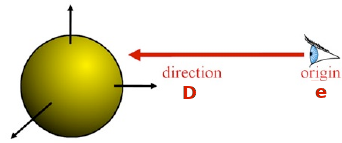
\includegraphics[width=3cm]{slike/ray_sfera.png}
\end{center}

Jednadžba:
$$(\textbf{p}(t)-x_c)^2 + (\textbf{p}(t)_y-y_c)^2 + (\textbf{p}(t)_z-z_c)^2 - R = 0$$
Vektorski, gdje je $\textbf{c}=(x_c, y_c, z_c)$:
$$(\textbf{p}(t)-\textbf{c})\cdot (\textbf{p}(t)-\textbf{c}) - R^2 = 0$$
$$(\textbf{e} + t\textbf{D}-\textbf{c})\cdot (\textbf{e} + t\textbf{D}-\textbf{c}) - R^2 = 0$$
\end{frame}	

\begin{frame}{Sjecište zrake i sfere, contd.}
$$(\textbf{e} + t\textbf{D}-\textbf{c})\cdot (\textbf{e} + t\textbf{D}-\textbf{c}) - R^2 = 0$$
Ako se sada izmnoži i uredi izraz, dobije se:

$$(\textbf{D}\cdot \textbf{D})t^2+2\textbf{D}\cdot(\textbf{e}-\textbf{c})t + (\textbf{e}-\textbf{c})\cdot(\textbf{e}-\textbf{c}) - R^2=0$$
Ako uvedemo supstituciju:\\
$A = \textbf{D}\cdot \textbf{D}$, $B = 2\textbf{D}\cdot(\textbf{e}-\textbf{c})$, $C = (\textbf{e}-\textbf{c})\cdot(\textbf{e}-\textbf{c}) - R^2$

$$t_{1,2} = \frac{-B \pm \sqrt{B^2-4AC}}{2A}$$

$\sqrt{B^2-4AC} < 0$ - nema sjecišta \\
Odabrati manji $t$, ali ako je negativan, ili manji od $d$ (udaljenost od očišta do prozora), znači da se sfera nalazi iza nas, odnosno između očišta i prozora.
\end{frame}	

\begin{frame}{Sjecište zrake i ravnine}
Pravac: $\textbf{p}(t) = \textbf{e}+t\textbf{D}$
\\Ravnina: točka na ravnini: $\textbf{p}_0 = (x_0, y_0, z_0)$, normala: $\textbf{n}$
\\Ako je točka na ravnini:\\
$(\textbf{p} - \textbf{p}_0)\textbf{n}=0$
ili:
$(\textbf{e} +t\textbf{D}- \textbf{p}_0)\textbf{n}=0$
\\Rješenje: $t = \frac{(\textbf{p}_0-\textbf{e})\cdot\textbf{n}}{\textbf{D}\cdot\textbf{n}}$

\begin{center}
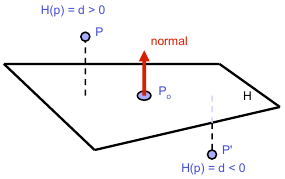
\includegraphics[width=4cm]{slike/ray_ravnina.png}
\end{center}
\end{frame}	

\begin{frame}{Sjecište zrake i ravnine, contd.}
Može i drugačije: Ako definiramo tri točke na ravnini, $(A, B, C)$ 
\begin{center}
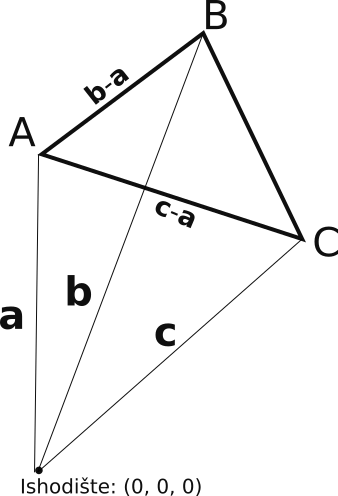
\includegraphics[width=2cm]{slike/ravnina_vector.png}
\end{center}
Točka na ravnini je zadana sa 
$\textbf{p}(\beta, \gamma) = \textbf{a} + \beta(\textbf{b}-\textbf{a}) + \gamma(\textbf{c}-\textbf{a})$
\end{frame}	

\begin{frame}{Sjecište zrake i ravnine, contd.}
$\textbf{p}(\beta, \gamma) = \textbf{a} + \beta(\textbf{b}-\textbf{a}) + \gamma(\textbf{c}-\textbf{a})$ 
\\
Ako je zadana zraka sa: $\textbf{p}(t) = \textbf{e}+t\textbf{D}$
$$\textbf{e}+t\textbf{D} = \textbf{a} + \beta(\textbf{b}-\textbf{a}) + \gamma(\textbf{c}-\textbf{a})$$
Dobije se sustav jednadžbi:
\begin{align*}
x_e+tx_D = x_a + \beta(x_b-x_a) + \gamma(x_c-x_a)\\
y_e+ty_D = y_a + \beta(y_b-y_a) + \gamma(y_c-y_a)\\
z_e+tz_D = z_a + \beta(z_b-z_a) + \gamma(z_c-z_a)
\end{align*}
Nepoznanice su $t$, $\beta$ i $\gamma$
\end{frame}	

\begin{frame}{Sjecište zrake i ravnine, contd.}
Nakon sređivanja prethodnog izraza:
\begin{align*}
(x_a-x_b)\beta + (x_a-x_c)\gamma + x_Dt=x_a-x_e\\
(y_a-y_b)\beta + (ya-y_c)\gamma + y_Dt=y_a-y_e\\
(z_a-z_b)\beta + (za-z_c)\gamma + z_Dt=z_a-z_e
\end{align*}
Odnosno:

\begin{align*}
\left[
\begin{array}{ccc}
x_a-x_b&  x_a-x_c&  x_D \\ 
y_a-y_b&  y_a-y_c&  y_D  \\ 
z_a-z_b&  z_a-z_c&  z_D
\end{array} 
\right]
\left[
\begin{array}{c}
\beta \\ \gamma \\ t
\end{array} 
\right] =
\left[
\begin{array}{c}
x_a-x_e \\ y_a-y_e \\ z_a-z_e
\end{array} 
\right]
\end{align*}
\end{frame}	

\begin{frame}{Sjecište zrake i ravnine, contd.}
Još jednostavnije:
\begin{align*}
\textbf{A}
\left[
\begin{array}{c}
\beta \\ \gamma \\ t
\end{array} 
\right] =
\left[
\begin{array}{c}
x_a-x_e \\ y_a-y_e \\ z_a-z_e
\end{array} 
\right]
\end{align*}
Zašto $\beta$ i $\gamma$?
\end{frame}

\begin{frame}{Sjecište zrake i ravnine, contd.}
Ravnina je zadana trima točkama $(A, B, C)$, ili pripadajućim vektorima $\mathbf{a}, \mathbf{b}, \mathbf{c}$.\\
Svaka točka $\mathbf{P}$ na ravnini se može zapisati kao  $\mathbf{P}(\alpha, \beta, \gamma) = \alpha\mathbf{a} + \beta\mathbf{b}+\gamma\mathbf{c}$, gdje je $\alpha + \beta +\gamma =1$
\begin{center}
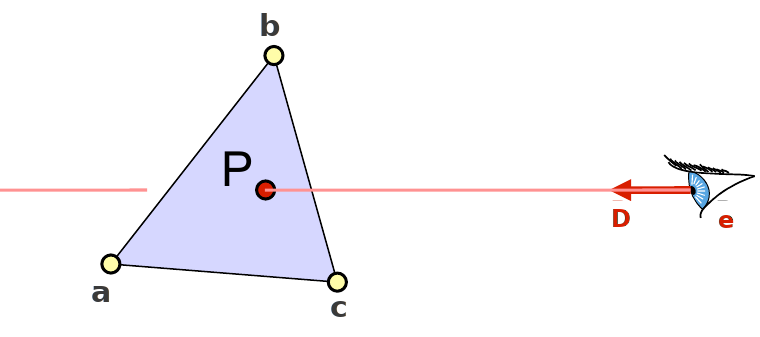
\includegraphics[width=5cm]{slike/ray_trokut_01.png}
\end{center}
Možemo izraziti $\alpha$ i drugačije: $\alpha = 1- \beta - \gamma$ \\
$\mathbf{P}(\beta, \gamma) = (1- \beta - \gamma)\mathbf{a} + \beta\mathbf{b}+\gamma\mathbf{c} = \mathbf{a} + \beta(\mathbf{b}-\mathbf{a}) + \gamma(\mathbf{c}-\mathbf{a})$\\
Dakle, izračunamo $t$, $\beta$ i $\gamma$ (pogledati slajdove iznad), onda dobijemo $\alpha$. \\
Ako vrijedi $\alpha + \beta +\gamma =1$, onda je točka na ravnini.
\end{frame}	


\begin{frame}{Sjecište zrake i trokuta}
Osim $\alpha + \beta +\gamma =1$, dodajemo još tri uvjeta $0 \leq \alpha \leq 1$, $0 \leq \beta \leq 1$, $0 \leq \gamma \leq 1$.\\
Primjer: 
\begin{itemize}
\item ako je $\alpha=0$, $\textbf{P}$ je na dužini $\textbf{b} - \textbf{c}$
\item ako je $\alpha=\beta=0$, $\textbf{P} = \textbf{c}$
\end{itemize}
Jednadžba koji treba riješiti:
$\textbf{p}(\beta, \gamma) = \textbf{a} + \beta(\textbf{b}-\textbf{a}) + \gamma(\textbf{c}-\textbf{a})$\\
ili:
\\ Jer je $\alpha = 1- \beta - \gamma$
Kako izračunati $\alpha, \beta, \gamma, t$?\\
Ako je zadana zraka sa: $\textbf{p}(t) = \textbf{e}+t\textbf{D}$, onda je jednadžba koju treba riješti:
$$\textbf{e}+t\textbf{D} = \textbf{a} + \beta(\textbf{b}-\textbf{a}) + \gamma(\textbf{c}-\textbf{a})$$
Primijetite da je jednadžba ista kao i za sjecište(probodište) zrake i ravnine. \\
Samo moramo provjeriti uvjet za trokut (na vrhu ovog slajda).


\end{frame}	

\section{Ray tracing}
\begin{frame}{Uvodno}
\begin{itemize}
	\item Neriješeni problemi 70-ih
	\begin{itemize}
		\item Sjene
		\item Refleksija
		\item Prozirnost
	\end{itemize}
	\item Turner Whitted - An improved illumination model for shaded display, 1979
\end{itemize}
\begin{figure}
	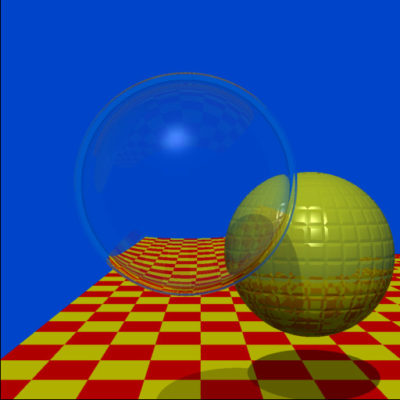
\includegraphics[width=0.4\textwidth]{./slike/whitted-spheres.jpg}
\end{figure}
\end{frame}

\begin{frame}{Pogled s visine}
\begin{tiny}
	Preuzeto sa \texttt{scratchapixel.com}
\end{tiny}

\begin{figure}
	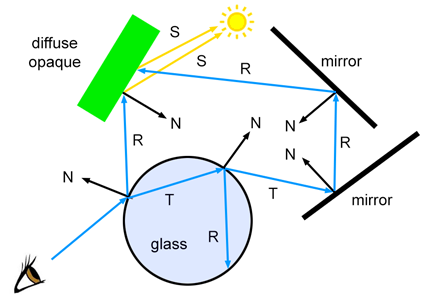
\includegraphics[width=0.4\textwidth]{./slike/rt-whitted-example}	
\end{figure}
Ako je u sjeni:
\begin{align*}
I = k_aI_a + \xcancel{I_i\left[k_d\left(\mathbf{n}\cdot\mathbf{l}\right)+
k_s\left(\mathbf{v}\cdot\mathbf{r}\right)^q\right]}
\end{align*}
Refleksija:
\begin{align*}
I = k_aI_a + I_i\left[k_d\left(\mathbf{n}\cdot\mathbf{l}\right)+
	k_s\left(\mathbf{v}\cdot\mathbf{r}\right)^q\right] + k_rI_o
\end{align*}
Prozirnost:
\begin{align*}
I = k_aI_a + I_i\left[k_d\left(\mathbf{n}\cdot\mathbf{l}\right)+
k_s\left(\mathbf{v}\cdot\mathbf{r}\right)^q\right] + k_tI_o
\end{align*}
\end{frame}

\begin{frame}{Pogled s visine}
\begin{figure}
	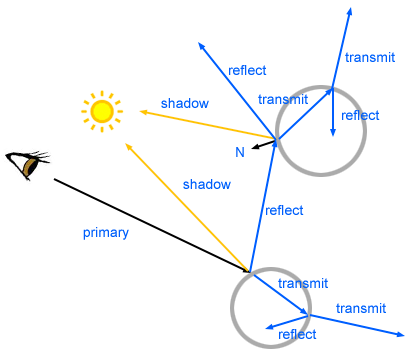
\includegraphics[width=0.8\textwidth]{./slike/rt-recursive}
\end{figure}
\tiny{Preuzeto sa \texttt{scratchapixel.com}}
\end{frame}

\section{Sjene}

\begin{frame}{Sjene}
\begin{center}
	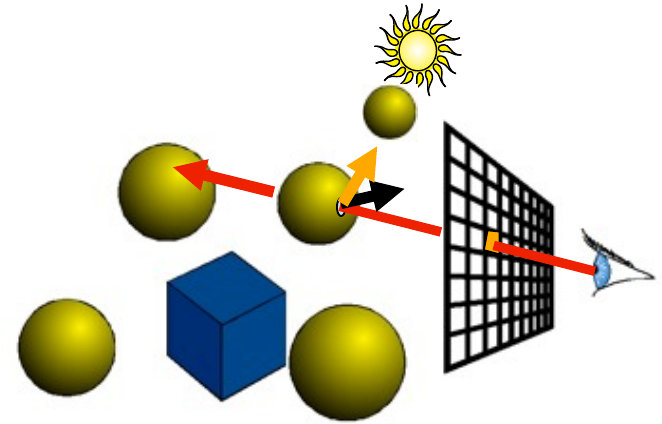
\includegraphics[width=8cm]{slike/sjene_01.png}
\end{center}

\end{frame}

\begin{frame}{Sjene, kostur algoritma}
\begin{algorithm*}[H]
%\KwResult{Write here the result }
color = ka*hit.material().kd()\;
\For{ za svaki izvor svjetla}
{
	Ray ray2(hitPoint, directionToLight)\;
	ambient = ka\;
	Hit hit2(distanceToLight)\;
	\For{ za svaki objekt}
	{
		object.intersect(ray2, hit2)\;
		%diffuseColor = object.intersect(ray2, hit2)\;
		\If{hit2->getT() == distanceToLight}
		{
			color += hit.getMaterial().shade(ray, hit, directionToLight, lightColor)\;
		}
	}
	
}
return color\;
%\caption{How to write algorithms}
\end{algorithm*}
\end{frame}

\begin{frame}{Sjene, contd.}
\begin{center}
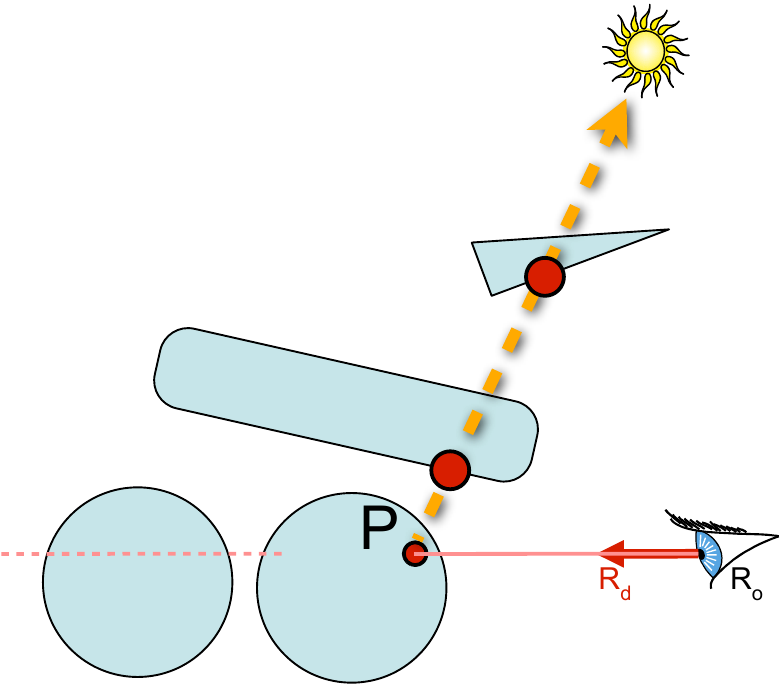
\includegraphics[width=4cm]{slike/sjene_02.png}
\end{center}
U čemu se razlikuju \textit{shadow} zrake u odnosu na \textit{eye} zrake?\\
Nije potrebno naći najbliži objekt, dovoljno je da je samo jedan između zrake i izvora svjetla 
\end{frame}

\section{Refleksija}
\begin{frame}{Refleksija}

\begin{center}
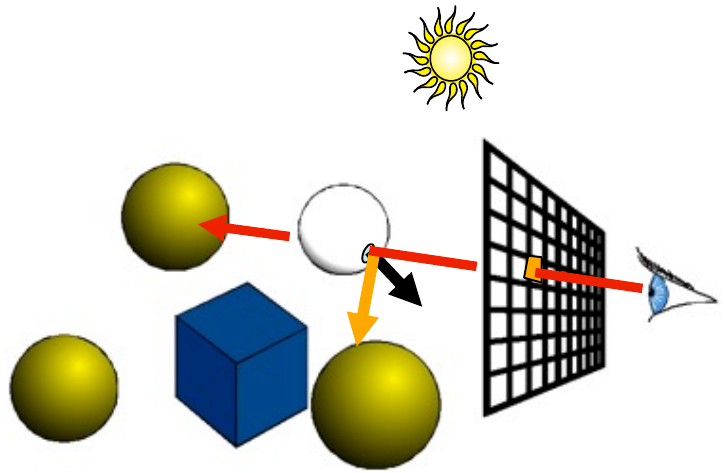
\includegraphics[width=5cm]{slike/refleksija_01.png}
\end{center}
\begin{itemize}
\item Odaslati zraku simetrično na normalu
\item pomnožiti sa zrcalnom komponentom $k_s$, ili nešto slično tome
\end{itemize}
\end{frame}

\begin{frame}{Refleksija, kako izračunati zrcalnu zraku}

\begin{center}
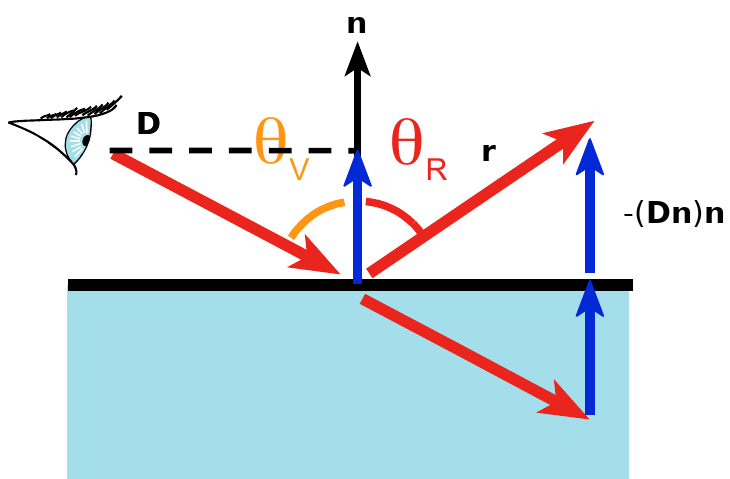
\includegraphics[width=6cm]{slike/refleksija_02.png}
\end{center}
$$\mathbf{r} = \mathbf{D} - 2(\mathbf{D}\cdot \mathbf{n})\mathbf{n}$$
\end{frame}


\section{Prozirnost}
\begin{frame}{Prozirnost}

\begin{center}
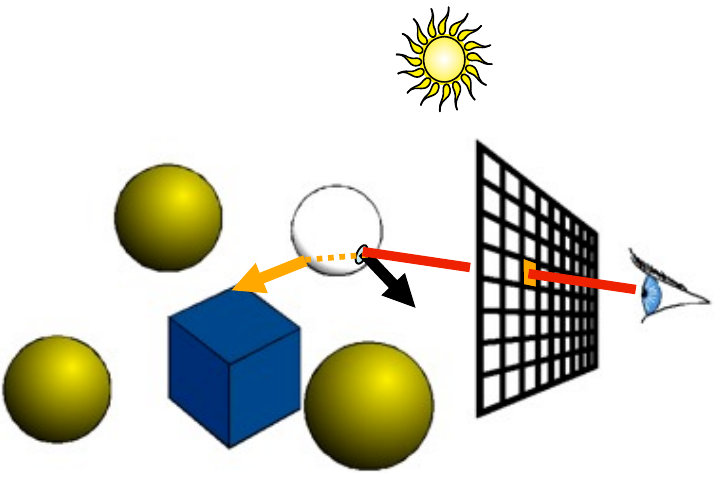
\includegraphics[width=5cm]{slike/prozirnost_01.png}
\end{center}
\begin{itemize}
\item Odaslati zraku u \textit{refrakcijskom} smjeru
\item pomnožiti s koeficijentom refrakcije $k_t$
\end{itemize}
\end{frame}

\begin{frame}{Prozirnost, contd.}

\begin{center}
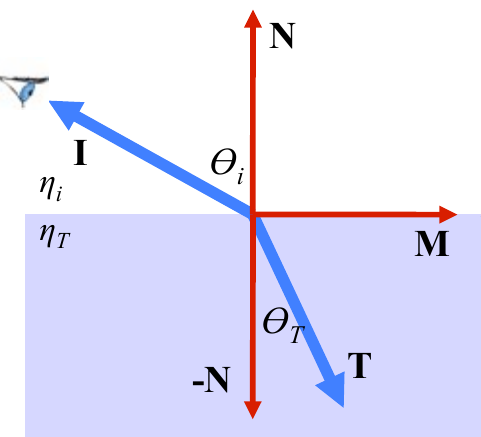
\includegraphics[width=3cm]{slike/prozirnost_02.png}
\end{center}
\begin{itemize}
\item dva materijala, dva indeksa refrakcije, $\eta_i$ i $\eta_t$
\end{itemize}
Snell-Descartes -ov zakon zakon:
$$\eta_i \theta_i = \eta_t \theta_t$$
$$\frac{\theta_t}{\theta_i} = \frac{\eta_t}{\eta_i} = \eta_r$$
Relativni indeks refrakcije: $\eta_r$\\
Cilj je odrediti smjer zrake $\mathbf{T}$
\end{frame}

\begin{frame}{Prozirnost, kako odrediti $\mathbf{T}$}
\begin{center}
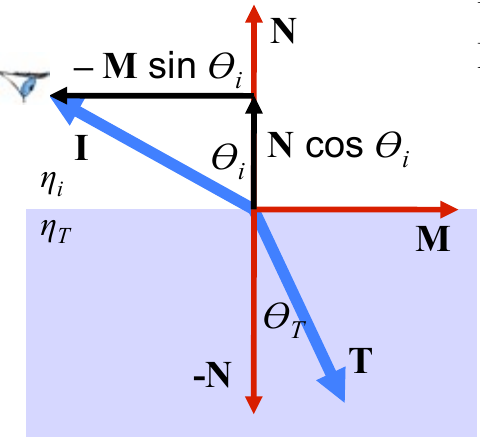
\includegraphics[width=3cm]{slike/prozirnost_03.png}
\end{center}
Odredimo $\mathbf{I}$ i $\mathbf{M}$:
\begin{align*}
\mathbf{I} &= \mathbf{N}\cos\theta_i - \mathbf{M}\sin\theta_i \\
\mathbf{M} &= (\mathbf{N}\cos\theta_i - \mathbf{I})/\sin\theta_i
\end{align*}
$\mathbf{T}$ je sada jednostavan:
$$ \mathbf{T} = -\mathbf{N}\cos\theta_t - \mathbf{M}\sin\theta_t $$
Cilj je izračunati $\mathbf{T}$ bez trigonometrijskih f-ja. Bilo bi super da možemo
koristiti samo skalarne produkte\ldots
\end{frame}

\begin{frame}{Prozirnost, kako odrediti $\mathbf{T}$, contd.}
\begin{align}
\mathbf{T} &= -\mathbf{N}\cos\theta_t + \mathbf{M}\sin\theta_t \\
&= -\mathbf{N}\cos\theta_t + ((\mathbf{N}\cos\theta_i - \mathbf{I})/\sin\theta_i)\sin\theta_t \\
&= -\mathbf{N}\cos\theta_t + (\mathbf{N}\cos\theta_i - \mathbf{I})\eta_r \\
&= \left(\eta_r\cos\theta_i - \cos\theta_t\right)\mathbf{N} - \eta_r\mathbf{I} \\
&= \left(\eta_r\cos\theta_i - \sqrt{1-\sin^2\theta_t}\right)\mathbf{N} - \eta_r\mathbf{I} \\
&= \left(\eta_r\cos\theta_i - \sqrt{1-\eta_r^2\sin^2\theta_i}\right)\mathbf{N} - \eta_r\mathbf{I} \\
&= \left(\eta_r\cos\theta_i - \sqrt{1-\eta_r^2(1-\cos^2\theta_i)}\right)\mathbf{N} - \eta_r\mathbf{I} \\
\mathbf{T} &= \left(\eta_r(\mathbf{N}\cdot \mathbf{I}) - \sqrt{1-\eta_r^2(1-(\mathbf{N}\cdot \mathbf{I})^2)}\right)\mathbf{N} - \eta_r\mathbf{I}
\end{align}
\end{frame}

\begin{frame}{Prozirnost, kako odrediti $\mathbf{T}$, contd.}
\begin{center}
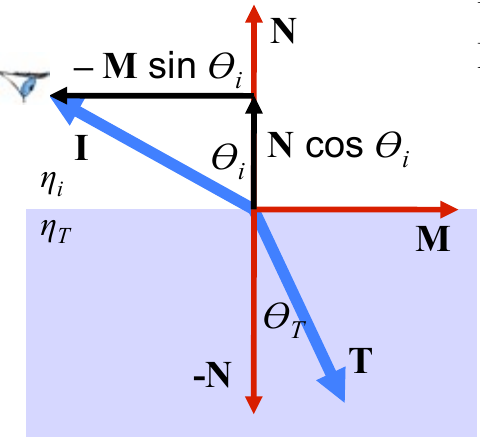
\includegraphics[width=3cm]{slike/prozirnost_03.png}
\end{center}
\begin{itemize}
\item  U izvodu smo prvo zamijenili $\mathbf{M}$ iz $\mathbf{M} = (\mathbf{N}\cos\theta_i - \mathbf{I})/\sin\theta_i$
\item uveli koeficijent refrakcije $\eta_r$
\item Iskoristili $\sin^2 \alpha + \cos^2 \alpha= 1$
\item Izrazili $\sin \theta_t$ pomoću $\sin \theta_i$
\item Na kraju iskoristili činjenicu da je $\mathbf{N}\cdot \mathbf{I}= \cos\theta_i$
\end{itemize}

\end{frame}
\plain{Pitanja?}
\end{document}